\chapter{Versionskontrolle Einführung - Git}

\section{Git}
\begin{itemize}
	\item Git = (engl.) Blödmann
	\item freie Software zur verteilten Versionsverwaltung von Dateien
	\item entwickelt für Quellcode-Verwaltung des Linus-Kernels
	\item Vokale Systeme: "Local Version Control Systems" (LVCS) -  SVN - Subversion \\
	\item Verteilte Systeme: "Distributed Version Control Systems" \\
	Mehrere verteilte Repositories für die zu archivierenden Dateien. 
	Bsp. Git \\
\end{itemize}

Ziele von Git
\begin{itemize}
	\item Geschwindigkeit
	\item Einfaches Design
	\item Vollständig verteilt (distributed Repository)
	\item Gute Unterstützung von nicht-linearer Entwicklung 
	\item ..
\end{itemize}

\subsection{Sicherungsart im Vergleich}
Git
\begin{itemize}
	\item stream of snapshots
	\item Speichert Snapshot von aktuellen Filesystem
	\item Link falls Datei nicht geändert (Pointer)
	\item Erst dann werden Deltas verwendet
\end{itemize}

SVN
\begin{itemize}
	\item Speichert die Datei beim ersten Mal und danach nur noch alle Änderungen
	\item Wird ein File aufgerufen, dann muss es erst das File erstellen und alle Änderungen durchführen
\end{itemize}

Bilder einfügen!

\subsection{Status von Dateien}
\begin{itemize}
	\item [committed:] Daten sicher gespeichert im lokalen Repo
	\item [modified:] Datei ist geändert zu (letztem Stand) aber nicht committed
	\item [staged:] Modifizierte Files ist markiert mit aktueller Version um im nächsten Commit-Snapshot zu gehen
	\item
\end{itemize}

\subsection{Bereiche}
\begin{itemize}
	\item Working Directory:
	\item Staging Area/ Index: 
	\item .git directory (lokal):
\end{itemize}

\subsection{Git Workflow}
Erstellen eines Ordners
\textbf{-mkdir gitTest} \\
Erstellen eines Git Repositories (.git Ordner):
\textbf{git init} \\
Erstellung eines lokalen Repositories erfolgt. \\

Tracked vs. Untracked: Dateien die Git bekannt sind. Die unter Versionsverwaltung stehen. 
Add the file
Edit the file
Stage the file
Commit the file
Remove the file

Übersicht über die aktuelle Lage im Repository: \textbf{git status} \\
Funktionalität: \\
Registerzustand aller Files, Aktueller lokaler Branch, Abweichungen vom entfernten Branch.

Hinzufügen eines Files, welches bereits in den entsprechenden Ordner gespeichert wurde: \textbf{git add <file name>} \\
Überprüfung der Aktion: \textbf{git status} \\
File dem Repository hinzufügen: \textbf{git commit -m "Comment"} \\
Fragt den Namen und die Email nach: \textbf{git config - global user} \\
Differenz zwischen Staging Area und Working Directory feststellen: \textbf{git diff <file name>} \\
Wiederum das File "stagen": \textbf{git add <file name>} \\
File dem Working Directory hinzufügen: \textbf{git commit -m "Comment"}
File aus der Versionsverwaltung raus nehmen: \textbf{git rm <file name"} \\
Histories anzeigen: \textbf{git log}

GUI: 
\begin{itemize}
	\item git gui
	\item gitk: "native gui" von git \\
	(Alle Branches werden angezeigt mit --all)
\end{itemize}

Commit Baum Darstellung: Jeder Commit hat einen eigenen Hash-Wert und es gibt dazu jeweils einen Snapshot. Branches sind Zeiger, die auf bestimmte Commits zeigen. Der Masterbranch zeigt auf den aktuellen Commit. 

Frühere Versionen zurückholen
Aus dem lokalen Repo wird etwas wieder in die Staging Area zurückgeholt: \textbf{git reset <path>} \\
Datei(en) "unstagen", indem die Dateiversion vom letzten Commit verwendet wird.  \\
Working Directory mit alter Version überschreiben: \textbf{git checkout HEAD path}

\subsection{git clone <URL>}
git clone https://git.hsr.ch/git/reponame
Beinhaltet folgende Schritte:
\begin{enumerate}
	\item Erstellt neues Verzeichnis
	\item Wechselt in das neu erstellte Verzeichnis
	\item Führt git init aus um lokales Repo zu erstellen
	\item Führt git remote add origin URL aus
	\item Führt git fetch aus
	\item Führt git checkout –b branch
	origin/branch ( HEAD vom remote Repo)
\end{enumerate}
Von einem entfernten Repo wird ein lokales Repo erstellt.

\subsection{git remote add <kurzname> <URL>}
Verbindung zu einem entfernten Repo erstellen. Bsp.: git remote add origin https://git.hsr.ch/git/gitTest \\
per default wird origin als Kurznamen für ein 
remote Repo verwendet \\
Normalerweise verwendet man git clone und nicht git remote. \\

\subsection{git fetch <remotename>}
Aktualisiert lokales Repo vom Remote Repo. Bsp.: git fetch origin. \\
Die Commits, die wir schon hatten bleiben, werden jedoch als "Branch" zur aktualisierten Version des Remote Repo, welche wir ins lokale Repo geladen haben, angezeigt. Nun hat man jedoch 2 Zweige, welche wieder vereint werden sollen. 

\subsection{git pull}
Aktualisiert lokales Repo vom entfernten Repo und merged Änderungen zum lokalen Repo. 
Ist wie git fetch, jedoch werden die 2 Zweige ineinander verwoben "merge". //
git pull origin master entspricht git fetch origin \& git merge origin/branchname
Merge-Konflikte: Identische Codezeilen wurden geändert -> Manuelle Überprüfung der 2 Versionen und Entscheid für eine Version. 
Es ist wichtig, dass man modified files zuerst committed bevor man einen pull macht.

\subsection{git push}
Veröffentlich lokales Repo und der master-Branch wird aktualisiert. 
git push <remotename> <branchname>


\section{Tagging}

\subsection{git tag}
Tags sind da, um spezifische Punke in der History zu taggen.

\begin{itemize}
	\item Lightweight Tag \\
	git tag -a v2.3
	\item Annotated Tags (Kommentierter Tag) \\
	git tag -a v1.3 -m "myComment"
\end{itemize}

\section{Branching}

Ein Branch ist ein verschiebbarer Zeiger
Es gibt HEAD-Zeiger und Tags.
Der Master Branch wird per Default erstellt.

\subsection{git branch <branchname>}
Erstellen eines neuen Branch.  Jedoch wird nicht auf diesen Branch gewechselt (Head bleibt stehen), 
git checkout <branchname> Head-Zeiger wird auf neuen Branch verschoben. 
Nun erfolgt ein commit auf einem Branch. 

git checkout master
Der Head-Zeiger ist wieder auf dem master-branch.
git commit - nun wird wieder etwas auf dem Master-branch committed. 
Es resultiert eine Verzweigung.

\subsection{git merge}
Zusammenführen von zwei Branches. Es gibt Fast-Forward merge: git merge <brachname>. Der master-branch-Zeiger wird entlang der Kette verschoben. Es resultiert kein Merge-Problem.
Three-way Merge: Merging-Konflikte sind möglich.
Git entscheidet selbst ob ein FF-merge oder ein three-way merge erfolgen soll.  \\
Mergekonflikte: \\
Mit GUI: KDiff3 mittels \textbf{mergetool} \\
Eine von beiden Dateien komplett verwenden: \textbf{git checkout \lbrack--theirs/--ours\rbrack}

\subsection{git reset}
Datei(en) «unstagen», indem die Dateiversion 
vom letzten commit verwendet wird \\
git reset path \\
git reset <filename>
\adjustbox{width=7cm}{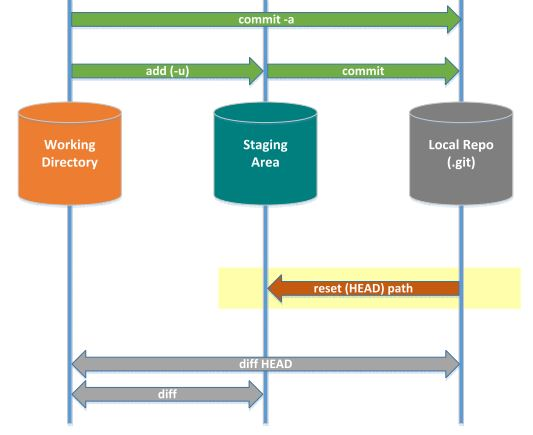
\includegraphics{Figures/reset}}

\subsection{git checkout}
Working Directory mit alter Version 
überschreiben: git checkout HEAD path \\

File(s) in  Staging Area wird von local Repo
überschrieben: git checkout <filename> \\

File(s) in Staging Area und Working Directory 
wird von local Repo überschrieben: git checkout HEAD README \\
Achtung: Kann Daten zerstören


\subsection{gitignore}

Hinzufügen von Files mit bestimmten Endungen zu gitignore: \\
echo *.aux >> .gitignore \\
Files verwerfen, die bereits in der Staged Area sind: \\
git rm --cached <filename>